\documentclass[../main.tex]{subfiles}

\begin{document}
	\section{Static Electricity}
		\begin{preamb}
			Static electricity is the study of charges at rest. In this chapter we will explore that very concept.
		\end{preamb}
		
		\pdef{Charge}{Charge is measured in coulombs [\si{\coulomb}]. There are positive and negative charges.}
		Like charges repel, unlike charges attract.
		\begin{center}
			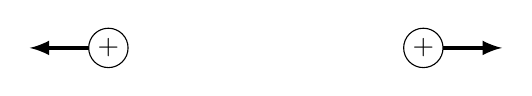
\begin{tikzpicture}
				\draw [line width=0.5mm, -latex] (-2,0) -- (-3,0);
				\draw [line width=0.5mm, -latex] (2,0) -- (3,0);
				\filldraw [fill=white] (-2,0) circle (0.25) node {\(+\)};
				\filldraw [fill=white] (2,0) circle (0.25) node {\(+\)};
			\end{tikzpicture}
		\end{center}
		\begin{center}
			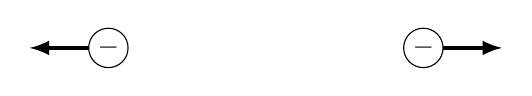
\begin{tikzpicture}
				\draw [line width=0.5mm, -latex] (-2,0) -- (-3,0);
				\draw [line width=0.5mm, -latex] (2,0) -- (3,0);
				\filldraw [fill=white] (-2,0) circle (0.25) node {\(-\)};
				\filldraw [fill=white] (2,0) circle (0.25) node {\(-\)};
			\end{tikzpicture}
		\end{center}
		\begin{center}
			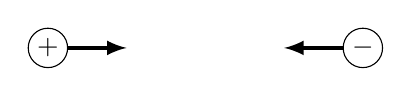
\begin{tikzpicture}
				\draw [line width=0.5mm, -latex] (-2,0) -- (-1,0);
				\draw [line width=0.5mm, -latex] (2,0) -- (1,0);
				\filldraw [fill=white] (-2,0) circle (0.25) node {\(+\)};
				\filldraw [fill=white] (2,0) circle (0.25) node {\(-\)};
			\end{tikzpicture}
		\end{center}
		
		\subsection{Electric Fields}
		
		\pdef{Electric Field}{An electric field is a region of space whereby a charge experiences an electric force.}
		
		\begin{center}
			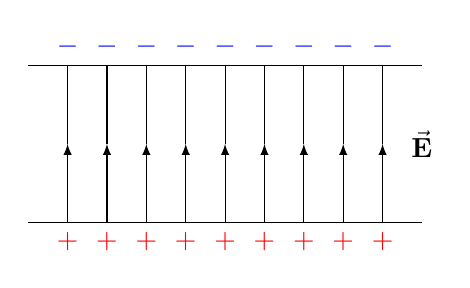
\begin{tikzpicture}
				\foreach \x in {1,...,9}
				\node [color=blue, anchor=south] at (0.5*\x,2) {\(-\)};
				\foreach \x in {1,...,9}
				\node [color=red, anchor=north] at (0.5*\x,0) {\(+\)};
				\node at (5,1) {\(\vec{\mathbf{E}}\)};
				\draw (0,0) -- (5,0);
				\draw (0,2) -- (5,2);
				\foreach \x in {1,...,9}
				\draw [-latex] (0.5*\x,0) -- (0.5*\x,1);
				\foreach \x in {1,...,9}
				\draw (0.5*\x,1) -- (0.5*\x,2);
			\end{tikzpicture}
		\end{center}
		
		\subsubsection{Isolated Charges}
		Field lines are the path a test charge would take within that electric field. The tighter the field lines are, the stronger the electric field at that area, which means that the test charge would experience a stronger force.
		
		Field lines extend \textbf{out} from \textbf{positive} charges.
		\begin{center}
			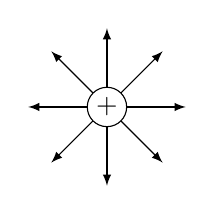
\begin{tikzpicture}
				\foreach \x in {0,...,7}
				\draw [-latex] (0,0) -- (45*\x:1);
				\filldraw [fill=white] (0,0) circle (0.25) node {\(+\)};				
			\end{tikzpicture}
		\end{center}
		Field lines go \textbf{in} to \textbf{negative} charges.
		\begin{center}
			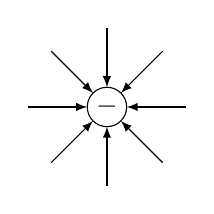
\begin{tikzpicture}
				\foreach \x in {0,...,7}
				\draw [latex-] (45*\x:0.25) -- (45*\x:1);
				\filldraw [fill=white] (0,0) circle (0.25) node {\(-\)};				
			\end{tikzpicture}
		\end{center}
		
		If a charge is stronger, it gets more field lines (e.g. this one has twice the charge as the one above, so it should get more)
		\begin{center}
			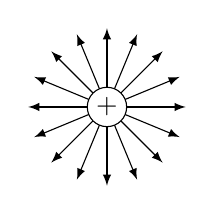
\begin{tikzpicture}
				\foreach \x in {0,...,15}
				\draw [-latex] (0,0) -- (22.5*\x:1);
				\filldraw [fill=white] (0,0) circle (0.25) node {\(+\)};				
			\end{tikzpicture}
		\end{center}
		
		Drawing these in TikZ was too difficult so take these from some online website.
		\begin{center}
			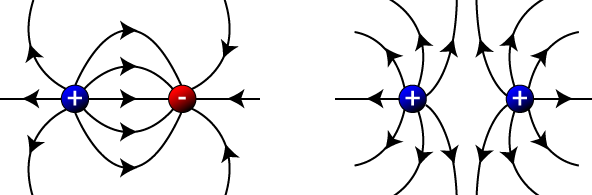
\includegraphics[width=\linewidth]{graphics/electrostaticsFieldLines}
		\end{center}
	
		\subsection{Charging}
		The two methods of charging are \textbf{rubbing} and \textbf{induction}.
		
		\subsubsection{Rubbing}
		Electrons (negative charges) can be transferred from one object to another through rubbing. There are no movement of positive charges.
		
		\subsubsection{Induction}
		Charging with induction can be achieved for two conductors. The most classic example is the metal sphere case.
		\begin{center}
			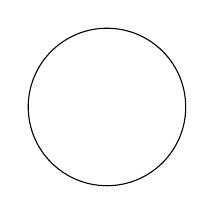
\begin{tikzpicture}
				\draw (0,0) circle (1cm);
			\end{tikzpicture}
		\end{center} 
		Suppose this sphere is overall neutral to begin with. Now a positively charged rod is brought to the sphere. This causes the electrons in the sphere to move towards the positively charged rod.
		\begin{center}
			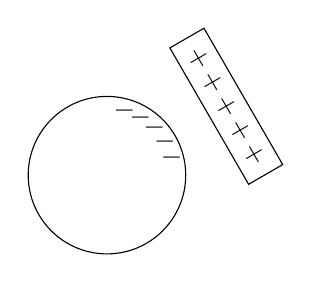
\begin{tikzpicture}
				\foreach \x in {15,30,45,60,75} \node at ({0.85*sin(\x)},{0.85*cos(\x)}) {\(-\)};
				\draw (0,0) circle (1);
				\draw[rotate=30] (1.5,-1) rectangle (2,1) node [pos=0.5, rotate=120]{\(+++++\)};
			\end{tikzpicture}
		\end{center} 
		The sphere is then earthed. Electrons flow from earth up to the sphere.
		\begin{center}
			\begin{circuitikz}
				\foreach \x in {15,30,45,60,75} \node at ({0.85*sin(\x)},{0.85*cos(\x)}) {\(-\)};
				\draw (0,0) circle (1);
				\draw[rotate=30] (1.5,-1) rectangle (2,1) node [pos=0.5, rotate=120]{\(+++++\)};
				\draw (-2,-1) node[ground] {} to (-2,{cos(225)}) -- ({sin(225)},{cos(225)});
				\draw[-latex] (-2,-1) -- (-2,{cos(225)-0.25}) node[anchor=east] {\(e^-\)};
			\end{circuitikz}
		\end{center} 
		The rod is then removed, leaving behind a negatively charged sphere.
		
		\subsection{Discharging}
		\subsubsection{Insulators}
		Insulators can be discharged by \textbf{heating} or \textbf{providing humid conditions}.
		
		\subsubsection{Conductors}
		Conductors can be discharged through a process known as \textbf{earthing}. Earthing allows electrons to flow into (in the case of a positively charged object) and out of (in the case of a negatively charged object) the object.
		\subsection{Applications and Hazards of Electrostatic Charging }
		\subsubsection{Applications}
		An application of electrostatics is in spray painting.
		
		In spray painting, the object to be painted is charged. The paint will then be charged with the opposite charge, and allowing the paint to attract to the object's surface, allowing for a better coat and efficient painting.
		
		\subsubsection{Hazards}
		Lightning is a danger that is caused by electrostatic charging.
		
		Charges build up in clouds due to friction between air and water molecules, which causes in ionised (charged) air which allows a conductive path between the charges built up in the clouds and ground, causing lightning.
		
		This can be resolved by installing conductive lightning rods on high objects such as buildings to safely ground these large releases of electric energy.
\end{document}
